\documentclass[hideothersubsections]{beamer}

\usepackage[francais]{babel}
\usepackage[utf8]{inputenc}
\usepackage[T1]{fontenc}

\usepackage{graphicx}
\usepackage{listings}
\usepackage{rotating}
\lstset{language=[objective]caml}   

\usetheme{Hannover}

\def\swidth{1.6cm}
\usenavigationsymbolstemplate{
	11 octobre 2013
	\hspace{0,3cm}
	GConfs - Conférence OCaml
	\hspace{0.3cm}
	Philémon GARDET 
	\hspace{0,3cm} 
	\large
	\insertframenumber/\inserttotalframenumber
}
\setbeamertemplate{sidebar left}{
	\vfill
	\insertverticalnavigation{\swidth}
	\vfill
}

\setcounter{tocdepth}{1}

\title{OCaml \\ De l'objet à l'utilisation de SDL}
\author{Philemon Gardet - Rafael Gozlan}
\institute{
\includegraphics[width=1.8cm]{pics/epita.png}\\
\includegraphics[width=2cm]{pics/gconfs.png}}
\date{11 octobre 2013}

\begin{document}
	\begin{frame}
		\titlepage
	\end{frame}

	\section*{Introduction}
\begin{frame}
	\frametitle{Les langages fonctionnels}
	
\includegraphics[width=9cm]{pics/history.png}
\end{frame}

\begin{frame}
	\frametitle{L'OCaml}
	\begin{itemize}
		\item OCaml est un langage fonctionnel...
		\item ... mais pas que : Imperatif et Orienté Objet
		\item Interprété mais aussi compilable en natif
		\item Peut être utilisé avec d'autres langages dans un projet
	\end{itemize}
\end{frame}


	\begin{frame}
		\tableofcontents
	\end{frame}

	\section{Rappels des bases d'OCaml}
\begin{frame}
  \begin{center}
	\huge
	La base, la sup, etc... et deux, trois, autres nouveautés !
  \end{center}
\end{frame}

\subsection{Les données de base} %%%%%%%%%%%%%%%%%%%%%%%%%%%%%%%
\begin{frame}[fragile]
	\frametitle{Les types élémentaires}
	\begin{itemize}
		\item Les entiers : 42\\
			~~4 * 10 + 2
		\item Les flottants : 4.2\\
			~~41.5 +. 0.5
		\item Les caractères : 'c'\\
		\item Les chaînes de caractères : "abcd"\\
			~~"The " \^~"meaning of " \^~"life"
			\item Les n-uplets : ( 1, 4.2, "abc", 4 )
		\item Le unit : ()
	\end{itemize}
\end{frame}

\begin{frame}[fragile]
	\frametitle{Les listes}
	\framesubtitle{Mais qu'est-ce que c'est ?}
	\begin{itemize}

	\item Liste vide:
		\begin{lstlisting}
		[]
		\end{lstlisting}

	\item Opérateur de construction:
		\begin{lstlisting}
		a :: []
		1 :: 2 :: 3 :: 4 :: 5 :: []
		"abc" :: "de" :: "f" :: "ghij" :: []
		\end{lstlisting}

	\item Concaténation (à éviter):
		\begin{lstlisting}
		liste1 @ liste2
		\end{lstlisting}

	\end{itemize}
\end{frame}

\begin{frame}[fragile]
	\frametitle{Les listes}
	\framesubtitle{Quelques fonctionnalités du module List}
	\begin{itemize}
	
	\item List.length : retourne la longueur d'une liste
	
	\item List.append : autre nom de l'opérateur @
	
	\item List.rev : inverse la liste passée en paramètre
	
	\item List.iter : application d'une fonction f à chacun des éléments de la liste

	\item List.map : renvoie une liste des résultats de l'application d'une fonction f à chacun des éléments de la liste

	\end{itemize}
\end{frame}


\subsection{Déclaration et fonctions} %%%%%%%%%%%%%%%%%%%%%%%%%%
\begin{frame}[fragile]
      \frametitle{Les déclarations}
      Il existe deux types de déclaration :
	\begin{columns}[t]
		\begin{column}{5cm}
		\begin{block}{Les globales}
		\begin{lstlisting}
	let a = "42";;
	val a : string = "42"
	\end{lstlisting}
	avec répétition :
	\begin{lstlisting}
	let a = 2
	and b = 3
	and c = 4;;
	val a : int = 2
	val b : int = 3
	val c : int = 4
		\end{lstlisting}
		\end{block}
		\end{column}
      		\begin{column}{5cm}
		\begin{block}{Les locales}
		\begin{lstlisting}
	let a = 2 in a + 1;;
	- : int = 3
	\end{lstlisting}
	avec répétition :
	\begin{lstlisting}
	let a = 2
	and b = 3
	and c = 4 in
	a + b + c;;
	- : int = 9
		\end{lstlisting}
		\end{block}
      		\end{column}
	\end{columns}
\end{frame}

\begin{frame}[fragile]
	\frametitle{Les fonctions}
	\framesubtitle{Représentation}
	\begin{center}
		\begin{minipage}{10cm}
				\begin{lstlisting}
     function x -> x + 1;;
     -: int -> int = <fun>
				\end{lstlisting}
				\begin{lstlisting}
     function x -> function y -> x + y;;
     - : int -> int -> int = <fun>
				\end{lstlisting}
				\begin{lstlisting}
     function (x , y) -> x * y;;
     - : int * int -> int = <fun>
				\end{lstlisting}
				\begin{lstlisting}
     fun x y -> x + y;;
     - : int -> int -> int = <fun>
				\end{lstlisting}
		\end{minipage}
  \end{center}
\end{frame}

\begin{frame}[fragile]
	\frametitle{Les fonctions}
  	\framesubtitle{Déclaration}
    	\begin{lstlisting}
	let name p1 pn = expr
    	\end{lstlisting}
	\begin{lstlisting}
let name =
  function p1 -> function pn -> expr
  	\end{lstlisting}
  	\vspace{0.4cm}
  	\begin{lstlisting}
let add x y = x + y;;
val add : int -> int -> int = <fun>
  	\end{lstlisting}
\end{frame}

\begin{frame}[fragile]
	\frametitle{Les fonctions}
	\framesubtitle{Déclaration récursive}
	\begin{block}{Déclaration de fonction récursive}
	  \begin{lstlisting}
	  let rec facto x =
	  	if x = 0 then 1 else x * facto(x-1);;
	  val facto : int -> int = <fun>
	  \end{lstlisting}
	\end{block}
\end{frame}

\begin{frame}[fragile]
	\frametitle{Les fonctions}
  	\framesubtitle{L'ordre supérieur}
  	Et si nous faisions des fonctions de fonctions ?
 	\begin{lstlisting}
  let comp f a b = f a b;;
  val comp : ('a -> 'b -> 'c) ->
  'a -> 'b -> 'c = <fun>

  comp (+) 3 2;;
  - : int = 5
 	\end{lstlisting}
	Nous retrouvons ici le type polymorphe, rassemblant tous les\\
	les types et representé par les 'a et 'b.
\end{frame}

\begin{frame}[fragile]
	\frametitle{Les fonctions}
	\framesubtitle{Les paramètres optionnels}	

	 	\begin{block}{Déclaration}
		\begin{lstlisting}
		  let incr ?step:(x = 1) r = r + x
		
		  val incr : ?step:int -> int -> int
		\end{lstlisting}
		\end{block}

	 	\begin{block}{Utilisation}
		\begin{lstlisting}
		  incr 32;;
		  - : int = 33
		  incr ~step:10 32
		  - : int = 42
		\end{lstlisting}
		\end{block}

\end{frame}

\subsection{Faire des choix} %%%%%%%%%%%%%%%%%%%%%%%%%%%%%%%%%%%
\begin{frame}[fragile]
	\frametitle{Le contrôle conditionnel}
	\begin{block}{La structure}
	\begin{lstlisting}
	  let f a b c =
	    if a
	     then b
	     else c

	  val f : bool -> 'a -> 'a -> 'a
	\end{lstlisting}
	\end{block}
	\begin{block}{'else' optionnel pour le type de retour unit}
	\begin{lstlisting}
	  let f a =
	    if a=42
	      then print_string "42!"
	      (* else () *)

	  val f : bool -> unit -> unit -> unit
	\end{lstlisting}
	\end{block}
\end{frame}

\begin{frame}[fragile]
    \frametitle{Les tests booléens}
	\begin{columns}
		\begin{column}{5cm}
			\begin{itemize}
				\item "not" : négation
				\item "\&\&" : ET logique
				\item "||" : OU logique
				\item "=" : egalité structurelle
				\item "<>" : négation de "="
			\end{itemize}
		\end{column}
		\begin{column}{5cm}
			\begin{itemize}
				\item "<" : inférieur strict
				\item ">" : supérieur strict
				\item "<=" : inférieur ou égal
				\item ">=" : supérieur ou égal
			\end{itemize}
		\end{column}
	\end{columns}
\end{frame}

\begin{frame}[fragile]
	\frametitle{Le filtrage de motif}
	\framesubtitle{Généralités}
	\begin{block}{La structure}
		\begin{lstlisting}
  match expr with
     m1 -> expr1
   | m2 -> expr2
   | mn -> exprn
		\end{lstlisting}
	\end{block}
	\begin{block}{Exemples}
		\begin{columns}
		\begin{column}{5cm}
		\begin{lstlisting}
  match i with
     0 -> expr1
   | 5 | 12 -> expr2
   | n -> exprn
		\end{lstlisting}
		\end{column}
		\begin{column}{5cm}
		\begin{lstlisting}
  function
      42 -> true
    | _ -> false
		\end{lstlisting}
		\end{column}
	\end{columns}
	\end{block}
\end{frame}

\begin{frame}[fragile]
	\frametitle{Le filtrage de motif}
	\framesubtitle{Récursion et listes}
		\begin{lstlisting}
  let rec printStrList l = match l with
      [] -> print_string "\n"
    | e::[] -> print_string (e ^ "\n")
    | e::q ->
      print_string(e ^ ", ");
      printStrList q
		\end{lstlisting}
\end{frame}

\begin{frame}[fragile]
  	\frametitle{Le filtrage de motif}
	\framesubtitle{'as' et 'when'}
  	\begin{block}{As}
    	\begin{lstlisting}
	  let rec fibo = function
 	    0 | 1 as n -> n
 	  | x -> fibo(x - 1) + fibo(x - 2);;
    	\end{lstlisting}
  	\end{block}
  	\begin{block}{When}
    	\begin{lstlisting}
  let is_inf = function
        x when x < 42 -> true
    	| _ -> false;;
    	\end{lstlisting}
  	\end{block}
\end{frame}

\subsection{Les types} %%%%%%%%%%%%%%%%%%%%%%%%%%%%%%%%%%%%%%%%%
\begin{frame}[fragile]
	\frametitle{Créer un type}
	\framesubtitle{Types simples}
	\begin{lstlisting}
  type name = typeToDefine

  type point = int * int

  let a = (3,7);;
  val a : int * int = (3,7)
  let (b:point) = (3,7);;
  val b : point = (3,7)

  type stringLabeledIntList =
    string * (int list)

  type funIntList = (int list) -> int
	\end{lstlisting}
\end{frame}

\begin{frame}[fragile]
	\frametitle{Créer un type}
	\framesubtitle{Types paramétrés}
	\begin{lstlisting}
  type ('nameTypeParameter1,
 	     'nameTypeParameterN)
   	    name =
         typeToDefine

  type ('valType) labeledList =
    string * ('valType list)
	\end{lstlisting}
\end{frame}


\begin{frame}[fragile]
	\frametitle{Créer un type}
	\framesubtitle{Types somme}
	\begin{columns}
		\begin{column}{5cm}
			\begin{lstlisting}
  type head =
    | King
    | Queen
    | Jack

  type cardFigure =
    | Ace
    | NumberCard of int
    | HeadCard of head
			\end{lstlisting}
		\end{column}
		\begin{column}{7cm}
			\begin{lstlisting}
  type cardColor =
    | Spade
    | Heart
    | Diamond
    | Club

  type card =
    cardColor * cardFigure
			\end{lstlisting}
		\end{column}
	\end{columns}
\end{frame}


\begin{frame}[fragile]
	\frametitle{Créer un type}
	\framesubtitle{Types enregistrements}
	\begin{itemize}
	\item Déclaration de type:
		\begin{lstlisting}
		  type pixel =
		  {
		     mutable r:float;
		     mutable g:string;
		     b:int;
		  }

		let p = { r=2.4; g="The Game"; b=255 }
		\end{lstlisting}
	\item Accès aux champs et modification de leur valeur :
		\begin{lstlisting}
			  p.b;;
			  -: int = 255
			  p.g <- "You Lose"
		\end{lstlisting}
	\end{itemize}
\end{frame}



\begin{frame}[fragile]
	\frametitle{Les exceptions}
	\begin{lstlisting}
 exception Help
 exception HelpNbErr of int
	\end{lstlisting}
	\begin{block}{Pour lever une exception :}
		\begin{lstlisting}
  raise Help
  raise (HelpNbErr 451)

  invalid_arg "element parameter"
  failwith "uninitialized Graphics"
		\end{lstlisting}
	\end{block}
	\begin{block}{Pour traiter une exception}
		\begin{center}
			\begin{minipage}{4.2cm}
				\lstset{basicstyle=\scriptsize}
				\begin{lstlisting}
try expr with
| Exc1 -> expr1
| Exc2 (v1,v2) -> expr2
| Excn -> exprn
				\end{lstlisting}
			\end{minipage}
			\begin{minipage}{5cm}
				\lstset{basicstyle=\scriptsize}
				\begin{lstlisting}
try expr with
| MyExc -> print_string "lol"
| Invalid_argument n ->
    print_string ("InvArg:"^n)
| Failure -> exit (-1)
				\end{lstlisting}
			\end{minipage}
		\end{center}
	\end{block}
\end{frame}

	\subsection{Le côté imperatif d'OCaml} %%%%%%%%%%%%%%%%%%%%%%
%\begin{frame}[fragile]
%  \frametitle{le noyaux imperatif}
%  \framesubtitle{les entrées-sorties}
%  les canaux : 
%  \begin{lstlisting}
%      open_in
%      open_out
%      close_in
%      close_out
%   \end{lstlisting}
%    ecriture et lecture :
%  \begin{minipage}[t]{4cm}
%   \begin{lstlisting}
%    input_line
%    intput
%    output
%   \end{lstlisting}
%  \end{minipage}
%  \begin{minipage}[t]{4cm}
%   \begin{lstlisting}
%    print_newline
%    print_string
%    read_line
%   \end{lstlisting}
%  \end{minipage}
%\end{frame}

\begin{frame}[fragile]
	\frametitle{Le sequençage}
		\begin{block}{Séparer des expressions}
		\begin{lstlisting}
  expr1;...;expr2
		\end{lstlisting}
		\end{block}
		\begin{block}{Faire des "blocs" de code}
		\begin{lstlisting}
    begin
    expr1; 
    .
    .
    .
    exprn
  end
		\end{lstlisting}
		\end{block}
\end{frame}

\begin{frame}[fragile]
    \frametitle{Les boucles}
    \begin{block}{La boucle for}
	\begin{lstlisting}
	for nom = expr1 to expr2 do 
	expr3
	done

	for nom = expr1 downto expr2 do
	expr3
	done
	\end{lstlisting}
      \end{block}
	\begin{block}{La boucle while}
	\begin{lstlisting}
	while expr1 < expr2 do
	expr3
	done
      \end{lstlisting}
  \end{block}
\end{frame}

	
\section{Quelques structures de données}
\subsection{Les enregistrements}

\begin{frame}
	\begin{center}
		\huge 
		Les structures de données
	\end{center}
\end{frame}


\begin{frame}[fragile]
	\frametitle{Enregistrements}
	\begin{itemize}
	\item Déclaration de type: 
		\begin{lstlisting}
		type pixel = 
		{ mutable  r:float ; mutable g:string 
		; b:int } 
		\end{lstlisting}
		Un champ mutable signifie qu'il peut être modifié.
	
	\item Modifiaction des champs de valeur:
		\begin{lstlisting}
			p.r <- 42.0;
			p.g <- "The Game"
		\end{lstlisting}
	\end{itemize}
\end{frame}


\begin{frame}[fragile]
	\frametitle{Les références}
	Une référence est considéré comme l'équivalent (selon l'INRIA) des pointeurs en OCaml.
	Déclaration:
	\begin{lstlisting}
		let a = ref 0

		let l = ref [];;
		val l : '_a list ref = {contents=[]}
	\end{lstlisting}
	Utilisation:
	\begin{lstlisting}
		!a ;;
		- : int = 0
		a := !a + 1 ;;
		- : unit = ()
	\end{lstlisting}

\end{frame}

\subsection{Les vecteurs}

\begin{frame}
	\frametitle{Les vecteurs}
	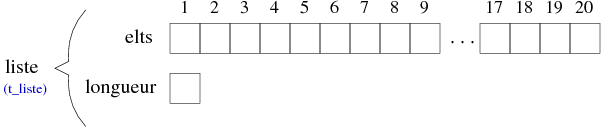
\includegraphics[scale=0.5]{pics/vect.png}
\end{frame}

\begin{frame}[fragile]
	\frametitle{Les vecteurs}
	\framesubtitle{Création}
	\begin{itemize}
	\item
	\begin{lstlisting}
	let v = [| 3.14; 6.28; 9.42 |];;
	val v : float array = [|3.14; 6.28; 9.42|]
	\end{lstlisting}

	\item Array.create
	\begin{lstlisting}
	let v = Array.create  3  3.14;;
	val v : float array = [|3.14; 3.14; 3.14|]
	\end{lstlisting}

	\item Array.make
	\end{itemize}
\end{frame}


\begin{frame}[fragile]
	\frametitle{Les vecteurs}
	\framesubtitle{Utilisation simple}
	\begin{enumerate}
	\item
	\begin{lstlisting}
	v.(1) ;;
	- : float = 3.14
	\end{lstlisting}

	\item
	\begin{lstlisting}
	v.(0) <- 100.0 ;;
	- : unit = ()
	\end{lstlisting}

	\item
	\begin{lstlisting}
	v ;;
	- : float array = [|100; 3.14; 3.14|]
	\end{lstlisting}
	\end{enumerate}
\end{frame}

\begin{frame}[fragile]
	\frametitle{Les vecteurs}
	\framesubtitle{Vecteur(ception)}
	\begin{lstlisting}
	let t = [| 
           [|1|];
           [|1; 1|];
           [|1; 2; 1|];
           [|1; 3; 3; 1|];
           [|1; 4; 6; 4; 1|];
           [|1; 5; 10; 10; 5; 1|]
         |] 
	\end{lstlisting}
\end{frame}

\begin{frame}[fragile]
	\frametitle{Les vecteurs}
	\framesubtitle{Copie et valeurs partagées}
	\begin{block}{Soit une copie simple}
	\begin{lstlisting}
	let v = Array.make 3 1;;
	val v : int array = [|1; 1; 1|]
	let m = Array.copy v ;;
	val m : int array = [|1; 1; 1|]

	v.(1)<- 1337;;
	- : unit = ()

	m;;
	-: int array = [|1; 1; 1|]
	\end{lstlisting}
	\end{block}
\end{frame}

\begin{frame}[fragile]
	\frametitle{Les vecteurs}
	\framesubtitle{Copie et valeurs partagées}
	\begin{block}{Et une copie avec valeurs partagées}
	\begin{lstlisting}
	let v = Array.make 3 1;;
	val v : int array = [|1; 1; 1|]
	let m = Array.make 3 v;;
	val m : int array array = 
	[|[|1; 1; 1|]; [|1; 1; 1|]; [|1; 1; 1|]|]
	let m2 = Array.copy m;;
	val m2 : int array array = 
	[|[|1; 1; 1|]; [|1; 1; 1|]; [|1; 1; 1|]|]
	v.(1)<- 1337;;
	- : unit = ()
	m2 ;;
	- : int array array = 
	[|[|1; 1337; 0|]; [|1; 1337; 0|]; 
	[|1; 1337; 0|]|]
	\end{lstlisting}
	\end{block}
\end{frame}


\begin{frame}[fragile]
	\frametitle{Les vecteurs}
	\framesubtitle{Autres fonctionnalitées du module Array}
	\begin{itemize}
	\item Array.make\_matrix
	
	\item Array.iter

	\item Array.map 

	\item Array.iteri

	\item Array.to\_list

	\item RTFM...

	\end{itemize}
\end{frame}


\begin{frame}
	\frametitle{Les piles}
	
\includegraphics[scale=0.4]{pics/stack.jpg}
\end{frame}

\begin{frame}[fragile]
	\frametitle{Les piles}
	\framesubtitle{Initialisation}
	Pour utiliser les piles en OCaml nous vous présenterons ici le module Stack (ensuite si ça vous amuse de les recoder...):
	\begin{lstlisting}
	open Stack
	\end{lstlisting}
	Pour créer une pile on utilise:
	\begin{lstlisting}
	let s = Stack.create ();;
	val s : '_a Stack.t = <abstr>
	\end{lstlisting}
\end{frame}

\subsection{Les piles}
\begin{frame}[fragile]
\frametitle{Les piles}
\framesubtitle{Utilisation}
	\begin{itemize}
	
	\item
		\begin{lstlisting}
		Stack.push "42" s; Stack.push s "1337";;
		- : unit = ()	
		\end{lstlisting}	
	
	\item
		\begin{lstlisting}
		Stack.pop s;;
		- : string = "43"
		Stack.top s;;
		- : string = "42"
		\end{lstlisting}	

	\end{itemize}

\end{frame}

\begin{frame}[fragile]
	\frametitle{Les piles}
	\framesubtitle{Les fonctions essentielles}
	\begin{itemize}
	
	\item
		\begin{lstlisting}
		Stack.clear
		\end{lstlisting}

	\item
		\begin{lstlisting}
		Stack.copy
		\end{lstlisting}	

	\item
		\begin{lstlisting}
		Stack.is_empty
		\end{lstlisting}	

	\item
		\begin{lstlisting}
		Stack.length
		\end{lstlisting}	

	\item
		\begin{lstlisting}
		Stack.iter
		\end{lstlisting}

	\end{itemize}

\end{frame}


	\section{La programmation orientée objet}
\begin{frame}
	\begin{center}
	\huge
	La programmation orientée objet
	\end{center}
\end{frame}

\subsection{Notion d'objet} %%%%%%%%%%%%%%%%%%%%%%%%%%%%%%%%%%%%%%%%%
\begin{frame}
	\frametitle{Comme une boite}
	\begin{center}
	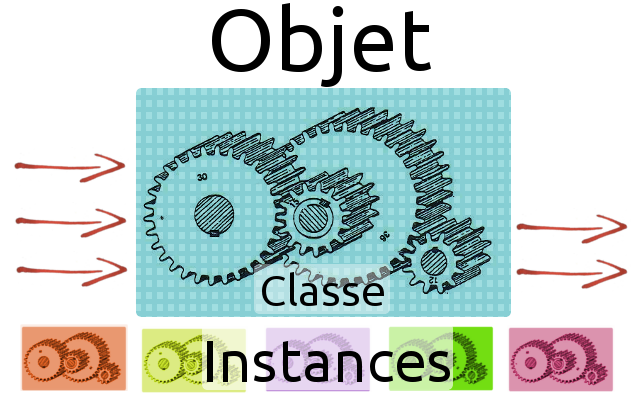
\includegraphics[width=9cm]{pics/explObj1.png}
	\end{center}
\end{frame}
\begin{frame}
	\frametitle{Attributs/Méthodes}
	\begin{center}
	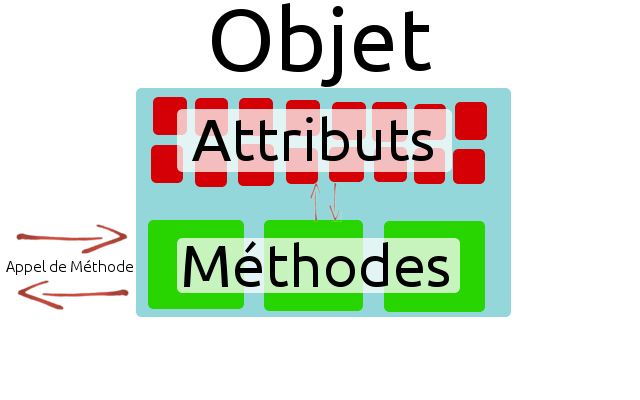
\includegraphics[width=9cm]{pics/explObj2.png}
	\end{center}
\end{frame}
\begin{frame}[fragile]
	\frametitle{Exemple d'utilisation d'objet}
	\begin{lstlisting}
let (c1,c2) =
  let m1 = new CoffeeMachine(Bresile)
  and m2 = new CoffeeMachine(Islande)
  in
  m1#addWater(1000);
  m2#addWater(42000);
  m1#headUp();
  m2#headUp();
  (m1#getCoffee(1),m2#getCoffee(3))
;;
	\end{lstlisting}
\end{frame}

\subsection{La déclaration d'un objet} %%%%%%%%%%%%%%%%%%%%%%%%%%%%%%
\begin{frame}[fragile]
	\frametitle{Syntaxe}
	\begin{minipage}{0.45\textwidth}
		\lstset{basicstyle=\small}
		\begin{lstlisting}
class name parameters =
  object
    (*Attributes*)

    (*Methods*)
  end
		\end{lstlisting}
	\end{minipage}
	\begin{minipage}{0.4\textwidth}
		\begin{lstlisting}
class point x y =
  object
    val x = x
    val y = y

    method printCoord =
      print_int x;
      print_string ",";
      print_int y;
      print_string "\n"
  end
		\end{lstlisting}
	\end{minipage}
\end{frame}

\begin{frame}[fragile]
	\frametitle{Déclaration d'attribut}
	\textit{Utilisez un type explicite pour les méthodes (pas de polymorphisme, pour l'instant...).}\\
	\begin{block}{Simple}
		\begin{lstlisting}
  val name = expr
		\end{lstlisting}
	\end{block}
	\begin{block}{Modifiable}
		\begin{lstlisting}
  val mutable name = expr
  name <- expr
		\end{lstlisting}
	\end{block}
	\begin{block}{Lorsque rien ne marche : Le type Option}
		\begin{lstlisting}
  val mutable name = None
  name <- Some expr
		\end{lstlisting}
	\end{block}
\end{frame}

\begin{frame}[fragile]
	\frametitle{Déclaration de méthode}
	\begin{block}{Publique}
		\begin{lstlisting}
  method name parameters = expr
		\end{lstlisting}
	\end{block}
	\begin{block}{Privée}
		\begin{minipage}{0.4\textwidth}
  			\begin{lstlisting}
  class name =
    object
    ...
    end
			\end{lstlisting}
		\end{minipage}$\Rightarrow$
		\begin{minipage}{0.4\textwidth}
			\begin{lstlisting}
  class name =
    object (self)
    ...
    end
			\end{lstlisting}
		\end{minipage}
	\end{block}
	\begin{lstlisting}
  method private name parameters = expr
  self#privateMethod parameters
	\end{lstlisting}
\end{frame}

\begin{frame}[fragile]
	\frametitle{Initialisation}
	\begin{lstlisting}
class putListInStack (l:int list) =
  object (self)

  val data = Stack.create ()

  initializer
    let rec storage = function
      | [] -> ()
      | e::q ->
        push e data;
        storage q
    in storage l

  ...
  end
	\end{lstlisting}
\end{frame}

\begin{frame}[fragile]
	\frametitle{Attributs polymorphiques}
	\begin{lstlisting}
class ['a] name parameters =
  object
  val data = ref []

  method add (e:'a) =
    data := e::!data

  ...
  end
	\end{lstlisting}
\end{frame}

\subsection{L'héritage} %%%%%%%%%%%%%%%%%%%%%%%%%%%%%%%%%%%%%%%%%%%%%
\begin{frame}[fragile]
	\frametitle{Héritage}
	\begin{lstlisting}
class childName parameters =
  object
  inherit parentClass parentsParameters

  end
	\end{lstlisting}
	\begin{lstlisting}
class childName parameters =
  object
  inherit parentClass parentsParameters
    as superParentClass

  end
	\end{lstlisting}
\end{frame}

\begin{frame}
	\frametitle{Accès aux méthodes de la classe mère 1/2}
	\lstinputlisting[firstline=1, lastline=14]{code/heritage.ml}
\end{frame}

\begin{frame}
	\frametitle{Accès aux méthodes de la classe mère 2/2}
	\textit{Le type d'une réécriture d'une méthode doit correspondre à celui de la méthode mère.}
	\textit{Pas de surcharge de fonction en OCaml}
	\lstinputlisting[firstline=16, lastline=28]{code/heritage.ml}
\end{frame}
\subsection{Le polymorphisme de sous-type} %%%%%%%%%%%%%%%%%%%%%%%%%%%
\begin{frame}
	\frametitle{Le polymorphisme de sous-type}
	\begin{center}
		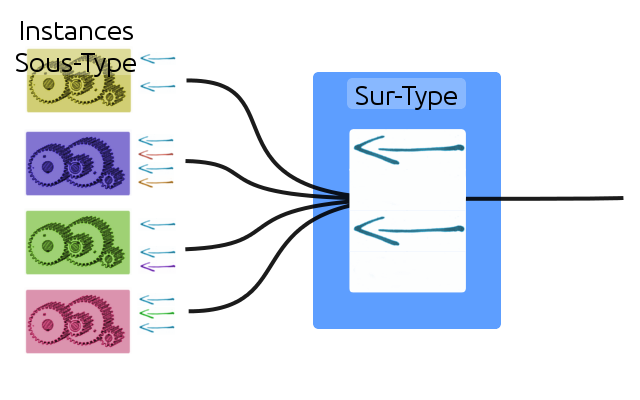
\includegraphics[width=9cm]{pics/inclusionObjet.png}
	\end{center}
\end{frame}

\begin{frame}[fragile]
	\frametitle{Interface et opérateur de sous-type}
	\framesubtitle{L'interface}
	\textit{On peut utiliser une classe ou une interface pour faire du polymorphisme de sous-type.}
	\begin{block}{Opérateur}
		~~Instance\_Sous-Type \large{:>} Sur-type
	\end{block}
	\begin{block}{Interface}
		\begin{lstlisting}
  class type interfaceName =
    object
      method mInterface1 : type1
      method mInferface2 : type2
    end
		\end{lstlisting}
	\end{block}
	\textit{Les types des méthodes doivent correspondre à ceux des méthodes de l'interface/classe.}
\end{frame}

\begin{frame}[fragile]
	\frametitle{Interface et opérateur de sous-type}
	\framesubtitle{Exemple d'utilisation}
	Réutilisons les class point et colored\_point.
	\begin{lstlisting}
let f (o:point) = o#setCoord 4 2
let test =
  ((new colored_point (4,2) 255):>point)

test#print;
f test;
test#print;
test#setData 4 5 1
	\end{lstlisting}
	\begin{block}{Sortie}
		\begin{lstlisting}
  (2,4) 255
  (4,2) 255
  Error: This expression has type point
         It has no method setData
		\end{lstlisting}
	\end{block}
\end{frame}

	\section[SDL]{La bibliothèque SDL}

\subsection{SDL} %%%%%%%%%%%%%%%%%%%%%%%%%%%%%%%%%%%%%%%%%%%%
\begin{frame}
	\begin{center}
		\huge
		La bibliothèque SDL
	\end{center}
\end{frame}

\begin{frame}
	\frametitle{Le principe actif SDL}
	\begin{center}
		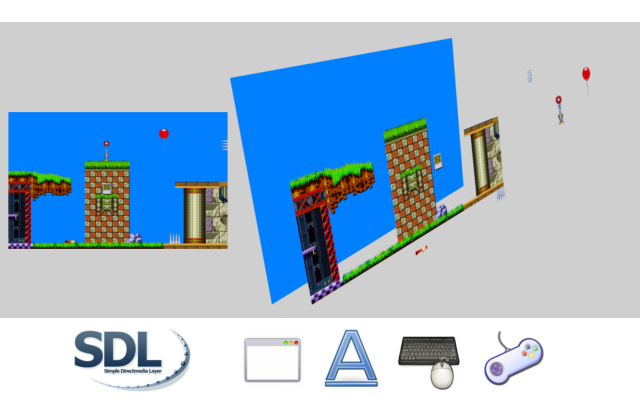
\includegraphics[width=9cm]{pics/sdlSurfaces.png}
	\end{center}
\end{frame}

\begin{frame}[fragile]
	\frametitle{Les modules SDL}
	\begin{columns}
		\begin{column}{3cm}
			\begin{itemize}
				\item Sdl
				\item Sdlwm
				\item Sdlvideo
				\item Sdltime
				\item Sdlevent
			\end{itemize}
		\end{column}
		\begin{column}{3cm}
			\begin{itemize}
				\item Sdlttf
				\item Sdlloader
				\item Sdlmixer
				\item Sdlgfx
			\end{itemize}
		\end{column}
	\end{columns}
\end{frame}

\subsection{Introduction à SDL} %%%%%%%%%%%%%%%%%%%%%%%%%%%%%%%%%%%%%%%%%%%%%%%
\begin{frame}[fragile]
	\frametitle{Initialisation de SDL}
	\begin{columns}
		\begin{column}{5cm}
			\begin{block}{L'initialisation de base}
				\lstset{basicstyle=\small}
				\begin{lstlisting}
  Sdl.init [`EVERYTHING] 
				\end{lstlisting}
			\end{block}
			\begin{block}{L'initialisation et ouverture d'une fenêtre}
				\lstset{basicstyle=\small}
				\begin{lstlisting}
  Sdl.init [`EVERYTHING]

  let screen = 
   Sdlvideo.set_video_mode 
   ~w ~h ~bpp [`HWSURFACE]
				\end{lstlisting}
			\end{block}
			\begin{block}{Quitter Sdl}
				\lstset{basicstyle=\small}
				\begin{lstlisting}
  Sdl.quit ()
				\end{lstlisting}
			\end{block}
		\end{column}
		\begin{column}{3.3cm}
			\begin{block}{types d'initialisation}
				\begin{itemize}
					\item `AUDIO
					\item `CDROM
					\item `JOYSTICK
					\item `TIMER
					\item `VIDEO
				\end{itemize}
				\begin{itemize}
					\item `EVERYTHING
				\end{itemize}
			\end{block}
		\end{column}
	\end{columns}
\end{frame}

\subsection{L'affichage bas niveau} %%%%%%%%%%%%%%%%%%%%%%%%%%%%%%%%%%%%%%%%%%%
\begin{frame}[fragile]
	\frametitle{Quelques mots sur les surfaces}
	\framesubtitle{Type de la surface}
	\begin{columns}
		\begin{column}{5.2cm}
			\begin{block}{Caractéristiques}
				\lstset{basicstyle=\small}
				\begin{lstlisting}
type surface_info = {
  flags : surface_flags list;
  w : int;
  h : int;
  pitch : int;
  clip_rect : rect;
  refcount : int;
}
				\end{lstlisting}
			\end{block}
		\end{column}
		\begin{column}{3.6cm}
			\begin{block}{Types}
				\begin{itemize}
					\item `FULLSCREEN
					\item `HWSURFACE
					\item `OPENGL
					\item `SWSURFACE
					\item `SRCALPHA
					\item `RESIZABLE
					\item `SRCCOLORKEY
					\item `DOUBLEBUF
				\end{itemize}
			\end{block}
		\end{column}
	\end{columns}
\end{frame}


\begin{frame}
	\frametitle{Quelques mots sur les surfaces}
	\framesubtitle{La surface de type \textit{Double Buffer}}
	\begin{center}
		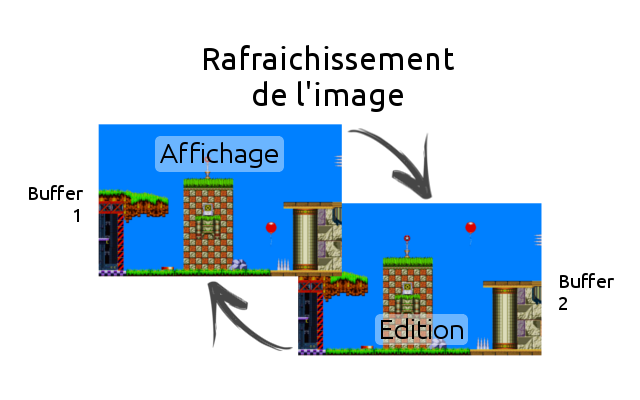
\includegraphics[width=9cm]{pics/doubleBuffer.png}
	\end{center}
\end{frame}

\begin{frame}[fragile]
	\frametitle{Quelques mots sur les surfaces}
	\framesubtitle{Le type rect}
	\begin{center}\begin{minipage}{0.4\textwidth}
		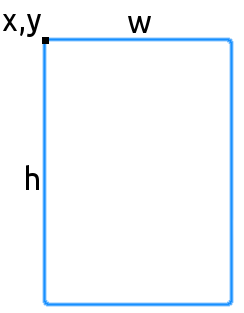
\includegraphics[width=3cm]{pics/rect.png}
	\end{minipage}
	\begin{minipage}{0.4\textwidth}
		\begin{block}{Position et dimentions}
			\lstset{basicstyle=\footnotesize}
			\begin{lstlisting}
  type rect = {
    mutable r_x : int;
    mutable r_y : int;
    mutable r_w : int;
    mutable r_h : int;
  } 
			\end{lstlisting}
		\end{block}
	\end{minipage}\end{center}
	\begin{block}{Fonctions liées}
		\lstset{basicstyle=\footnotesize}
		\begin{lstlisting}
  val rect : x:int -> y:int -> w:int -> h:int -> rect

  val surface_dims : surface -> int * int * int
		\end{lstlisting}
	\end{block}
\end{frame}

\begin{frame}[fragile]
	\frametitle{Le chargement d'image}
	\begin{block}{Charger/Sauver une image .bmp}
		\begin{lstlisting}
  val load_BMP : string -> surface

  val save_BMP : surface -> string -> unit
		\end{lstlisting}
	\end{block}
	\begin{block}{Charger une image .jpeg .png .tiff}
		\begin{lstlisting}
  val Sdlloader.load_image : string -> surface

		\end{lstlisting}
	\end{block}
\end{frame}

\begin{frame}
	\frametitle{Les pixels}
	\begin{center}
		
\includegraphics[width=9cm]{pics/Joconde-pixel.jpg}
	\end{center}
\end{frame}

\begin{frame}[fragile]
	\frametitle{Les pixels}
	\framesubtitle{La couleur}
	\begin{block}{Types}
		\textit{La couleurs peut être sous la forme d'un color ou d'un int32.}
		\begin{lstlisting}
  type color = int * int * int
  let c = ((255,255,255):color)
		\end{lstlisting}
	\end{block}
	\begin{block}{Fonctions de convertions}
		\begin{lstlisting}
  val map_RGB : surface -> ?alpha:int -> 
    color -> int32
  val get_RGB : surface -> int32 -> color
  val get_RGBA : surface -> int32 -> 
    color * int
		\end{lstlisting}
	\end{block}
\end{frame}

\begin{frame}[fragile]
	\frametitle{Les pixels}
	\framesubtitle{La transparance des surfaces}
	\begin{block}{Couleur transparante}
		\begin{lstlisting}
  val get_color_key : surface -> int32
  val set_color_key : surface -> ?rle:bool -> 
    int32 -> unit
  val unset_color_key : surface -> unit
		\end{lstlisting}
	\end{block}
	\begin{block}{Transparance globale}
		\begin{lstlisting}
  val get_alpha : surface -> int
  val set_alpha : surface -> ?rle:bool -> 
    int -> unit
  val unset_alpha : surface -> unit
		\end{lstlisting}
	\end{block}
\end{frame}

\begin{frame}[fragile]
	\frametitle{Les pixels}
	\framesubtitle{\og{}Bon ! Quand est-ce qu'on manipule des pixels ?\fg}
	\begin{block}{Vérouillage de la surface}
		\begin{lstlisting}
  val lock : surface -> unit
  val unlock : surface -> unit
  val must_lock : surface -> bool
		\end{lstlisting}
	\end{block}
	\begin{block}{Modification de la surface}
		\begin{lstlisting}
  val get_pixel : surface -> x:int -> 
    y:int -> int32

  val put_pixel : surface -> x:int -> 
    y:int -> int32 -> unit
		\end{lstlisting}
		\textit{Existe aussi en version prenant le format color au lieu du int32. Pour cela ajouter le suffixe \_color à la fonction.}
	\end{block}
\end{frame}

\begin{frame}[fragile]
	\frametitle{\og{}Merge Down !\fg}
	\begin{center}
		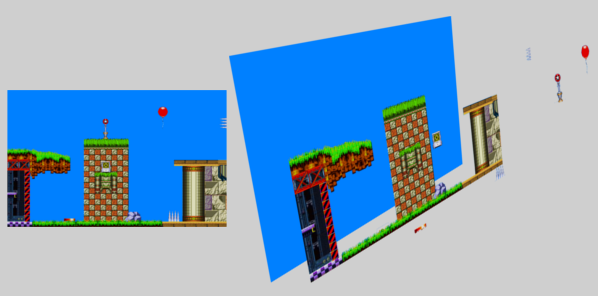
\includegraphics[width=3.6cm]{pics/surfacesMerge.png}
	\end{center}
	\begin{block}{Écraser/faire un fond de couleur}
		\begin{lstlisting}
  val fill_rect : ?rect:rect -> surface -> 
    int32 -> unit
		\end{lstlisting}
	\end{block}
	\begin{block}{Coller une surface sur une autre}
		\begin{lstlisting}
  val blit_surface : src:surface -> 
    ?src_rect:rect ->  dst:surface -> 
    ?dst_rect:rect -> unit -> unit
		\end{lstlisting}
	\end{block}
\end{frame}

\begin{frame}[fragile]
	\frametitle{L'actualisation de l'affichage}
	\framesubtitle{Surface Utilisateur}
	\begin{center}
		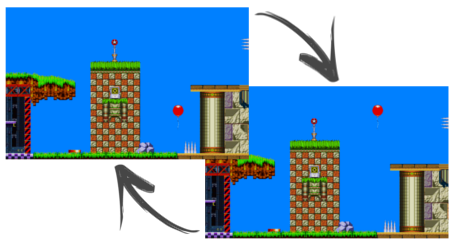
\includegraphics[width=2.4cm]{pics/doubleBufferScreen.png}
	\end{center}
	\begin{block}{La surface \og{}Fenêtre utilisateur\fg}
		\begin{lstlisting}
  val set_video_mode : w:int -> 
    h:int -> ?bpp:int -> 
    video_flag list -> surface
  val get_video_surface : unit -> 
    surface
		\end{lstlisting}
	\end{block}
	
\end{frame}

\begin{frame}[fragile]
	\frametitle{L'actualisation de l'affichage}
	\framesubtitle{Rafraîchissement de la surface utilisateur}
	\begin{center}
		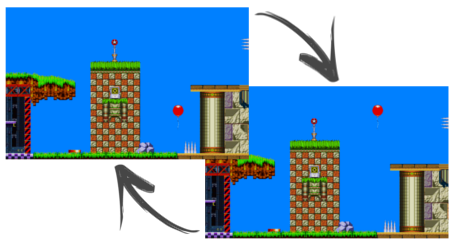
\includegraphics[width=2.4cm]{pics/doubleBufferScreen.png}
	\end{center}
	\begin{block}{Fonction de rafraîchissement}
		\begin{lstlisting}
  val update_rect : ?rect:rect -> 
    surface -> unit
  val update_rects : rect list -> 
    surface -> unit
		\end{lstlisting}
	\end{block}
	\begin{block}{Rafraîchissement pour un \textit{Double Buffer}}
		\begin{lstlisting}
  val flip : surface -> unit
		\end{lstlisting}
	\end{block}
\end{frame}

\begin{frame}[fragile]
	\frametitle{Créer des surfaces à partir de rien}
	\lstset{basicstyle=\footnotesize}
	\begin{lstlisting}
val create_RGB_surface_format : surface ->
  [ `ASYNCBLIT | `HWSURFACE | `SRCALPHA 
  | `SRCCOLORKEY | `SWSURFACE ] list ->
  w:int -> h:int -> surface

val create_RGB_surface : 
  [ `ASYNCBLIT | `HWSURFACE | `SRCALPHA 
  | `SRCCOLORKEY | `SWSURFACE ] list ->
  w:int -> h:int -> bpp:int ->
  rmask:int32 -> gmask:int32 -> bmask:int32 ->
  amask:int32 -> surface
	\end{lstlisting}
\end{frame}

\subsection{La détection d'événement} %%%%%%%%%%%%%%%%%%%%%%%%%%%%%%%%%%%%%%%%%
\begin{frame}[fragile]
	\frametitle{Détecter et récupérer un événement}
	\begin{block}{Attendre l'utilisateur}
		\begin{lstlisting}
  val wait_event : unit -> event
		\end{lstlisting}
	\end{block}
	\begin{block}{Traite la file des derniers événements}
		\begin{lstlisting}
  val poll : unit -> event option
		\end{lstlisting}
	\end{block}
\end{frame}

\begin{frame}[fragile]
	\frametitle{Les differents types d'événement}
	\lstset{basicstyle=\small}
	\begin{lstlisting}
type event =
| ACTIVE of active_event
| KEYDOWN of keyboard_event
| KEYUP of keyboard_event
| MOUSEMOTION of mousemotion_event
| MOUSEBUTTONDOWN of mousebutton_event
| MOUSEBUTTONUP of mousebutton_event
| JOYAXISMOTION of joyaxis_event
| JOYBALLMOTION of joyball_event
| JOYHATMOTION of joyhat_event
| JOYBUTTONDOWN of joybutton_event
| JOYBUTTONUP of joybutton_event
| QUIT
| SYSWM
| VIDEORESIZE of int * int
| VIDEOEXPOSE
| USER of int
	\end{lstlisting}
\end{frame}

\begin{frame}[fragile]
	\frametitle{Sous-événement Clavier/Souris}
	\lstset{basicstyle=\scriptsize}
	\begin{block}{Clavier}
		\begin{lstlisting}
  type keyboard_event = {
    ke_which : int;
    ke_state : switch_state;
    keysym : Sdlkey.t;
    keymod : Sdlkey.mod_state;
    keycode : char;
    unicode : int;
  }
		\end{lstlisting}
	\end{block}
	\begin{block}{Souris}
		\begin{minipage}{0.47\textwidth}
			\begin{lstlisting}
  type mousemotion_event = {
    mme_which : int;
    mme_state : 
      Sdlmouse.button list;
    mme_x : int;
    mme_y : int;
    mme_xrel : int;
    mme_yrel : int;
  }
			\end{lstlisting}
		\end{minipage}
		\begin{minipage}{0.4\textwidth}
			\begin{lstlisting}
  type mousebutton_event = {
    mbe_which : int;
    mbe_button : 
      Sdlmouse.button;
    mbe_state : switch_state;
    mbe_x : int;
    mbe_y : int;
  }
			\end{lstlisting}
		\end{minipage}
	\end{block}
\end{frame}

\subsection{Une boucle Sdl classique} %%%%%%%%%%%%%%%%%%%%%%%%%%%%%%%%%%%%%%%%%
\begin{frame}[fragile]
	\frametitle{Gestion des événements}
	\begin{lstlisting}
let updateEvent () = 
  match Sdlevent.poll () with
  | None -> ()
  | Some (Sdlevent.KEYDOWN key) -> 
    keyDownManager key
  | Some (Sdlevent.MOUSEBUTTONDOWN button) -> 
    buttonDownManager button
  | Some Sdlevent.QUIT -> Sdl.quit ()
  | _ -> ()
	\end{lstlisting}
\end{frame}

\begin{frame}[fragile]
	\frametitle{Modification et déplacement des élement visuels}
	\lstset{basicstyle=\scriptsize}
	\begin{lstlisting}
val blit_surface : src:surface -> ?src_rect:rect -> 
  dst:surface -> ?dst_rect:rect -> unit -> unit
	\end{lstlisting}
	\textit{Soit displayData une file de fonction Sdlvideo.blit\_surface dont tout les paramètres sont renseignés sauf le unit final}
	\lstset{basicstyle=\normalsize}
	\begin{lstlisting}
let updateDisplay () = 
  while not (is_empty displayData) do
    (take displayData) ()
  done
	\end{lstlisting}
\end{frame}

\begin{frame}[fragile]
	\frametitle{Actualisation}
	\begin{lstlisting}
let update () =
  let ticks = (*17ms -> 60fps *) 
    17 + Sdltimer.get_ticks () 
  in
  updateEvent();
  updateDisplay();
  while (Sdltimer.get_ticks ()) <= ticks do 
    () done
	\end{lstlisting}
\end{frame}

	\section{Organisation d'un projet}

\begin{frame}
	\begin{center}
		\huge
		Organisation d'un projet
	\end{center}
\end{frame}

\subsection{Les modules} %%%%%%%%%%%%%%%%%%%%%%%%%%%%%%%%%%%%%%%%%%%%%%%%%%%%%%
\begin{frame}
	\frametitle{Principe des modules}
	\begin{center}
		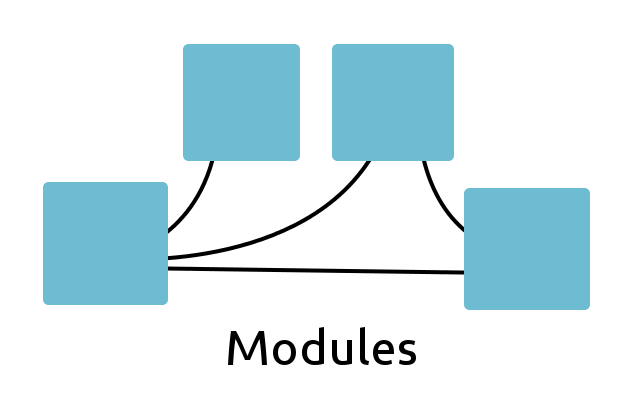
\includegraphics[width=9cm]{pics/modules.png}
	\end{center}
\end{frame}

\begin{frame}[fragile]
	\frametitle{Utilisation de fonctions d'un module}
	\begin{center}
		\begin{minipage}{0.5\textwidth}
			\begin{lstlisting}
open List

length 
  (1::3::3::7::[])
			\end{lstlisting}
		\end{minipage}
		\begin{minipage}{0.4\textwidth}
			\begin{lstlisting}
List.length 
  (1::3::3::7::[])
			\end{lstlisting}
		\end{minipage}
	\end{center}
\end{frame}

\begin{frame}
	\frametitle{Une facon de creer un module : Un fichier...}
	\begin{center}
		\begin{minipage}{0.5\textwidth}
			main.ml\\
			processing.ml\\
			rotation.ml\\
			cutting.ml\\
			recongition.ml
		\end{minipage}
		\begin{minipage}{0.4\textwidth}
			processing.mli\\
			rotation.mli\\
			cutting.mli\\
			recongition.mli
		\end{minipage}
	\end{center}
\end{frame}

\begin{frame}[fragile]
	\frametitle{Les fichiers surface}
	\begin{center}
		\begin{minipage}{0.34\textwidth}
			someFunctions.ml
			\begin{lstlisting}
let add a b = 
  a + b

let addf a b = 
  a +. b

let sub a b = 
  a - b

let subf a b = 
  a -. b
			\end{lstlisting}
		\end{minipage}
		\begin{minipage}{0.5\textwidth}
			someFunctions.mli
			\begin{lstlisting}
val add : 
  int -> int -> int

val addf : 
  float -> float -> float

val sub :
  int -> int -> int

val subf :
  float -> float -> float
			\end{lstlisting}
		\end{minipage}
	\end{center}
\end{frame}

\begin{frame}[fragile]
	\frametitle{Syntaxe d'un fichier interface 1/3}
	\lstset{basicstyle=\small}
	\begin{lstlisting}
val f : int -> int -> int

exception badSurface of (int -> int) * int

type card =
| Ace
| Number of int
| Head of HeadCard

type coloredPoint = {
  pos : int * int;
  mutable color;
}
	\end{lstlisting}
\end{frame}

\begin{frame}[fragile]
	\frametitle{Syntaxe d'un fichier interface 2/3}
	\lstset{basicstyle=\small}
	\begin{lstlisting}
class counter :
  object
    val mutable i : int
    method getCounts : unit -> int
  end

class point :
  int * int -> 
    object
      val pos : int * int
      method printCoord : unit -> unit
    end

class ['a] storage = 
  object val mutable data : 'a list method addData : 'a -> unit end
	\end{lstlisting}
\end{frame}

\begin{frame}[fragile]
	\frametitle{Syntaxe d'un fichier interface 3/3}
	\lstset{basicstyle=\small}
	\begin{lstlisting}
class ['a] storage = 
  object 
    val mutable data : 'a list
    method addData : 'a -> unit 
  end
	\end{lstlisting}
\end{frame}


\subsection{Faire de la documentation} %%%%%%%%%%%%%%%%%%%%%%%%%%%%%%%%%%%%%%%%
\begin{frame}
	\frametitle{La documentation}

\end{frame}

\begin{frame}
	\frametitle{ocamldoc}

\end{frame}

\begin{frame}
	\frametitle{La position des commentaires}

\end{frame}

\subsection{La compilation avec ocamlbuild} %%%%%%%%%%%%%%%%%%%%%%%%%%%%%%%%%%%
\begin{frame}
	\frametitle{Les differentes sorties d'OCaml}

\end{frame}

\begin{frame}
	\frametitle{Un Makefile rustique}

\end{frame}

\begin{frame}
	\frametitle{ocamlbuild}

\end{frame}

\begin{frame}
	\frametitle{Inclure des bibliotheques}

\end{frame}

	\section*{Conclusion}

\begin{frame}
	\frametitle{Récapitulatif des notions abordées}
	\large
	\begin{center}
	'OCaml' 'Fonctionnel'
	'Types' 'Bibliothèques Standard' 'Objet' 'Polymorphisme de Sous-Type' 'Bibliothèque Sdl' 'Application Graphique' 'Modularité' 'Compilation'
	'Documentation'
	\end{center}
\end{frame}

\begin{frame}
	\frametitle{Quelques liens}
	\begin{block}{Documentations OCaml}
		\begin{itemize}
			\item http://caml.inria.fr/pub/docs/manual-ocaml-4.01/
			\item http://caml.inria.fr/pub/docs/manual-ocaml-4.01/libref

			\item http://www.pps.univ-paris-diderot.fr/Livres/ora/DA-OCAML/
		\end{itemize}
	\end{block}
	\begin{block}{Documentation SDL}
		\begin{itemize}
			\item http://ocamlsdl.sourceforge.net/doc/html
			\item http://www.libsdl.org/release/SDL-1.2.15/docs
		\end{itemize}
	\end{block}
	\begin{block}{Documentation ocamlbuild}
		\begin{itemize}
			\item http://caml.inria.fr/pub/docs/manual-ocaml-4.01/ocamlbuild.html
		\end{itemize}
	\end{block}
\end{frame}

\end{document}
